\documentclass[11pt,a4paper]{article}
\usepackage[left=2cm,text={17cm,25cm},top=2cm]{geometry}
\usepackage[T1]{fontenc}
\usepackage[czech]{babel}
\usepackage[utf8]{inputenc}
\usepackage{url}
\usepackage{graphicx}
\usepackage{pdfpages}
\usepackage{algorithmicx}
\graphicspath{ {img/} }

\begin{document}

\begin{center}
	\LARGE{Paralelní a distribuované algoritmy -- dokumentace k projektu 1}\\
	\large{Vysoké učení technické v Brně}
	\vspace{0.2cm}

	Petr Stehlík <xstehl14@stud.fit.vutbr.cz>     \today

\end{center}

\section{Zadání}

Cílem projektu byla implementace algoritmu enumeration sort na lineárním poli procesorů, který byl prezentován během přednášek. Běh a kompilace programu je zprostředkován pomocí skriptu \texttt{test.sh}. Implementace využívá knihovny Open MPI\cite{bib:openmpi}.


\section{Rozbor a analýza algoritmu}

Enumeration sort je algoritmus pro seřazení všech prvků $x_1...x_n$ pomocí nalezení konečné pozice všech prvků v poli. Toho algoritmus docílí pomoci porovnání všech prvků $x_i$ navzájem a určením kolik ostatních prvků je menších než daný prvek $x_i$.

Enumeration sort na lineárním poli procesorů disponuje společnou sběrnicí pro všechny procesory. Tato sběrnice je schopna v každém kroku přenést jednu hodnotu a všechny procesory jsou doplněny lineárním spojením. Schéma zapojení procesorů je znázorněné na obrázku \ref{schema}.

Každý procesor obsahuje celkem 4 registry: \textit{C} -- počet prvků menších než $x_i$, \textit{X} -- prvek $x_i$, \textit{Y} -- postupně prvky $x_1 ... x_n$, \textit{Z} -- seřazený prvek $Y_i$.

\begin{figure}[h]
    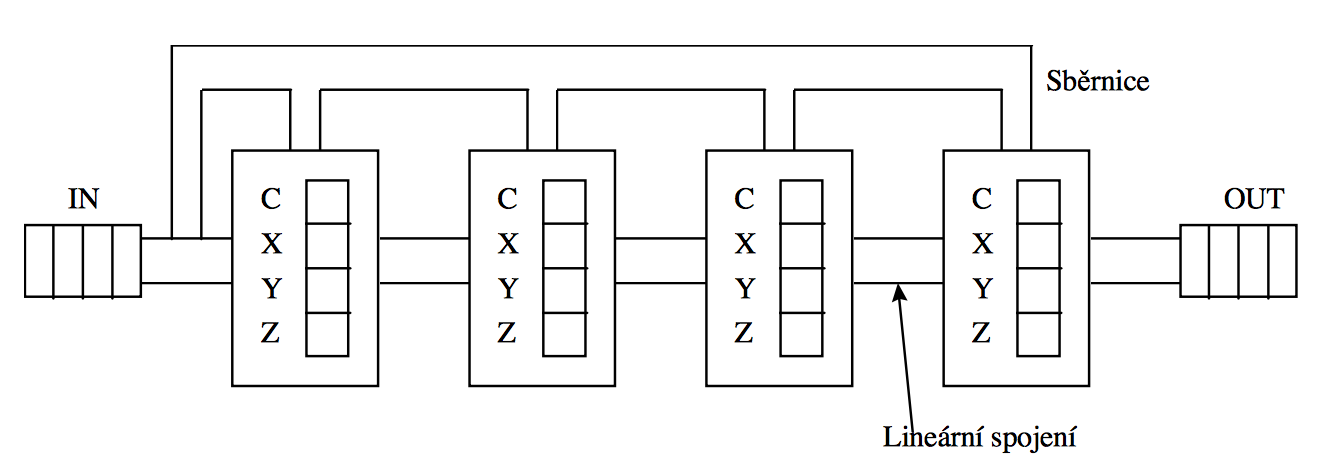
\includegraphics[width=0.7\linewidth]{schema}
    \centering
    \caption{Schéma zapojení procesorů. Převzato z \cite{bib:schema}}
    \label{schema}
\end{figure}

Algoritmus byl modifikován tak, aby dokázal řadit i duplicitní prvky. Pořadí u duplicitních prvků je určeno dle indexu porovnávaných identických prvků a adekvátně inkrementován registr $C$. Tato modifikace vychází z algoritmu popsaného v \cite{bib:sushi}.

\subsection{Algoritmus}
\begin{enumerate}
    \item {Všechny registry C nastaví na hodnotu 1}
    \item {Následující činnosti opakuj $2n$ krát, kde $1 \leq k \leq 2n$.}
        \begin{itemize}
            \item{Pokud není vstup vyčerpán, vstupní prvek $x_i$ se vloží přes sběrnici do registru $X_i$ a pomocí lineárního spojení do registru $Y_1$; obsah všech registrů $Y$ se posune doprava.}
            \item{Každý procesor s neprázdnými registry $X$ a $Y$ je porovná, a je-li $X > Y$ inkrementuje svůj registr $C$. Pokud $X = Y$, porovná index procesoru s indexem prvku v registru $Y$.}
			\item{Je-li $k > n$ (po vyčerpání vstupu) procesor $P_{k-n}$ pošle sběrnicí obsah svého registru $X$ procesoru $P_{C_{k-n}}$, který jej uloží do svého registru $Z$.}
        \end{itemize}
	\item{V následujících $n$ cyklech procesory posouvají obsah svých registrů $Z$ doprava a procesor $P_n$ produkuje seřazenou posloupnost.}
\end{enumerate}

\subsection{Analýza algoritmu}
Časová analýza jednotlivých kroků algoritmu: \textit{Krok 1} proběhne v konstatním čase, \textit{Krok 2} trvá $2n$ kroků, \textit{Krok 3} trvá n kroků.

Z těchto poznatků plyne $t(n) = \mathcal{O}(n)$ a k výpočtu potřebujeme n procesorů ($p(n)$). Celková cena algoritmu je tedy $c(n) = \mathcal{O}(n^2)$, což značí, že algoritmus enumeration sort není optimální.

\section{Implementace}

Algoritmus byl implementován za pomoci knihovny Open MPI v jazyce C++. Při inicializaci program vytvoří $n+1$ procesorů, kde procesor $P_0$ řídí vstup a výstup programu, rozesílá načtená čísla výpočetním procesorům a vypisuje je.

Po načtení čísla $x_k$ velikosti 1 bajt ze souboru \texttt{numbers} procesorem je číslo vypsáno na standardní výstup oddělené mezerou. Dále je číslo sběrnicí posláno procesoru $P_k$, uloženo do registru $X$ a lineárním spojením je posláno procesoru $P_1$ a uloženo do registru $Y$. Takto procesor $P_0$ zpracuje celý soubor.

Procesory $P_1 ... P_{n+1}$ jsou výpočetní procesory. Na sběrnici očekávají jedno číslo $x$ a pokud přijmou číslo $y$ přes lineární spojení, vyjmou ze svého registru Y číslo, odešlou jej svému sousedovi $P_{i+1}$ (vyjma procesoru $P_{n+1}$, ten číslo $y$ zahodí) a do registru $Y$ zapíšou nové číslo $y$. Sběrnice i lineární spojení je realizováno pomocí zasílání zpráv.

Pokud má procesor neprázdné registry $X$ a $Y$, poté při každém přijetí čísla $y$ provede porovnání registru $X$ a $Y$ a adekvátně inkrementuje registr $C$. Následně zkontroluje rovnost těchto čísel. Pokud ano, provede kontrolu interně vedeného čítače duplicit čísla $x$. Pokud je těchto duplicit $>1$, porovná index čísla $y$ a rank procesoru a upraví registr $C$ dle algoritmu. Index čísla $y$ je zasílán společně s číslem $Y$.

Po dokončení čtení a rozeslání všech čísel procesorem $P_0$ a po přenesení všech čísel skrze lineární spojení jsou po sběrnici rozeslány čísla $x$ procesoru s rankem odpovídající hodnotě $c$. Procesory toto číslo uloží do registru $Z$.

Následně jsou čísla z registru poslána svému sousedovi s nižším rankem. Procesor $P_0$ je tiskne na výstup, dokud nejsou všechna čísla poslána procesoru $P_0$.

\section{Experimentální ověření časové složitosti}

Experimety probíhaly na stroji disponujícím Intel(R) Core(TM) i7-2635QM CPU @ 2.00GHz, 8 GB RAM a SSD. Pro každý počet prvků byl test spuštěn $10x$ a doba běhu zprůměrována. Čas výpočtu byl měřen pomocí Open MPI funkce \texttt{Wtime()}.

\begin{figure}[!ht]
    \centering
		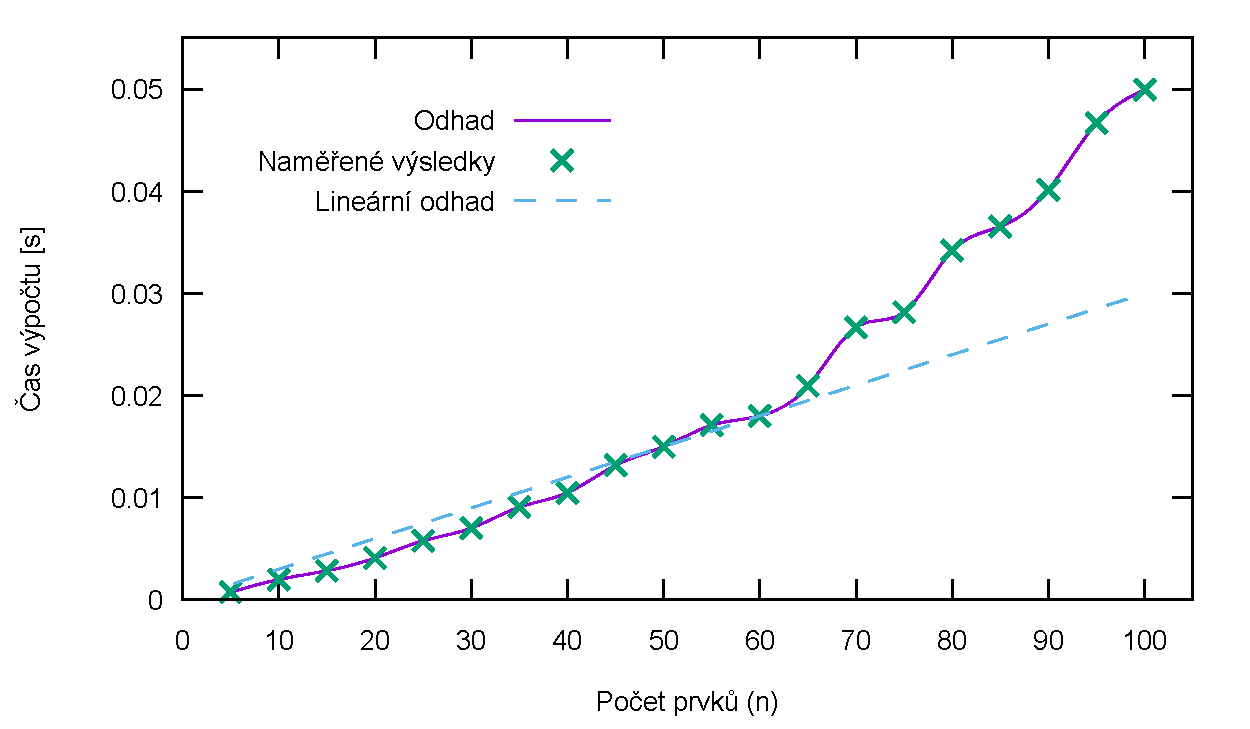
\includegraphics[width=0.6\textwidth]{results}
    \caption{Experimentálně naměřené výsledky}
\end{figure}

\section{Komunikační protokol}
\label{proto}

Protokol je znázorněn na obrázku \ref{proto_schema}. Zasílání zpráv je realizováno výhradně funkcemi \texttt{Send}, \texttt{Isend}, \texttt{Recv} a \texttt{Irecv} z knihovny Open MPI.

\begin{figure}[!h]
    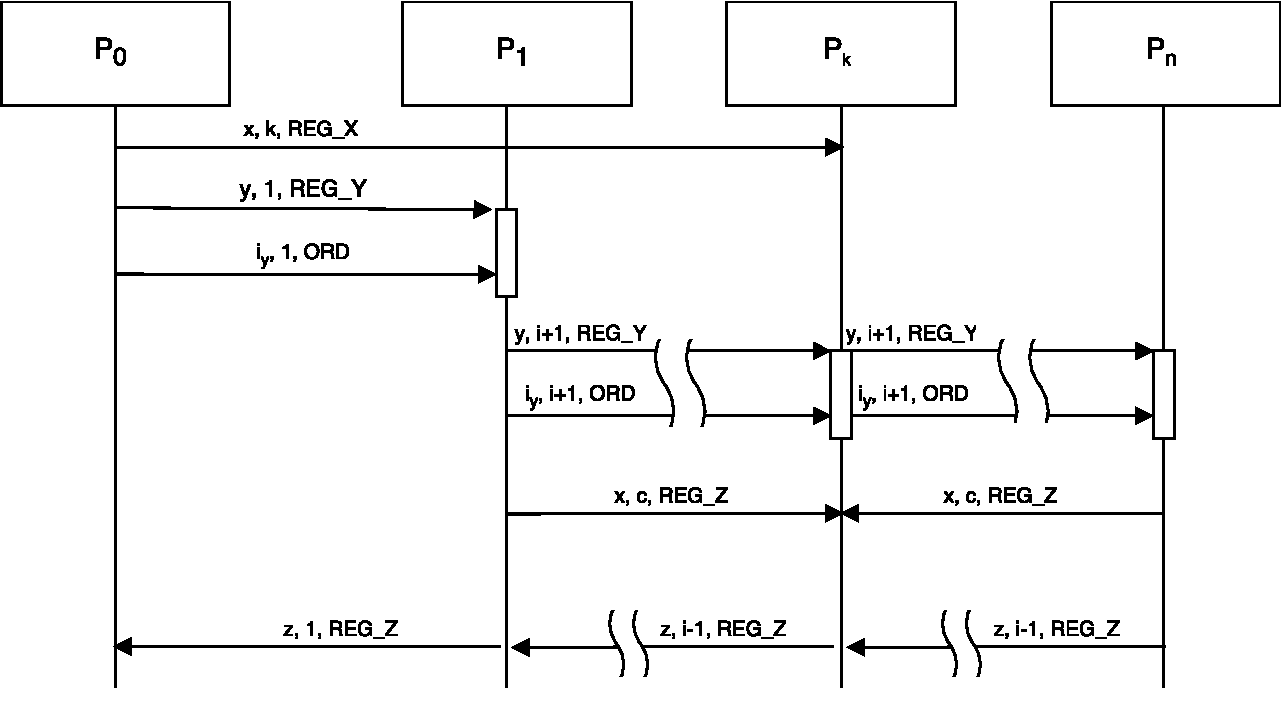
\includegraphics[width=0.7\linewidth]{protokol}
    \centering
    \caption{Sekvenční diagram komunikačního protokolu. Popisky obsahují následující informace: obsah registru, rank, tag.}
    \label{proto_schema}
\end{figure}


\section{Závěr}

Algoritmus se podařilo úspěšně implementovat a experimentálně otestovat. Algoritmus byl upraven tak, aby řadil i duplicitní hodnoty. Z naměřených výsledků lze usoudit, že algoritmus má lineární časovou složitost. Výsledky s více než 65 prvky těmto předpokládám neodpovídají kvůli zvýšené režii při přepínání procesů.


\bibliography{literature}

\makeatletter
\makeatother
\bibliographystyle{czechiso}

\end{document}

